\documentclass[12pt,oneside,openany,a4paper, %... Layout
afrikaans,english,
%... Global lang drivers
]{memoir}
\usepackage[report, goldenblock]{usthesis}%... Thesis options
\usepackage[afrikaans, english]{babel}

\usepackage{amsmath}
\usepackage{mathtools}
\numberwithin{equation}{chapter}
\usepackage{bm}
\usepackage{graphicx}
\usepackage{subcaption}
\usepackage{color} % or xcolor
\usepackage{float} %figure location

\renewcommand{\thesection}{\thechapter.\arabic{section}}
\usepackage{tabto}

%Watermark
\usepackage{eso-pic}
\newcommand*{\WaterMark}[2][0.15\paperwidth]{%
\AddToShipoutPicture*{\AtTextCenter{%
\parbox[c]{0pt}{\makebox[0pt][c]{%
\includegraphics[width=#1]{#2}}}}}}

%References
\usepackage{usbib}%............................. Bibliography
\bibliographystyle{usmeg-n}%................. Auhor-year style
\addto{\captionsenglish}{\renewcommand{\bibname}{List of References}}

\begin{document}
\pagestyle{plain}
\frontmatter
%TiltePage:
\title{Numerical integration for probabilisitc reasoning skripsie}
\author{JM.\ Louw}{Jacobus Martin Louw}
\faculty{Faculty of Electrical and Electronic Engineering}
\degree{BEng (E&E)}{Bachelor of Engineering (Electrical and Electronic)}
\ReportDescript{Final Report}
\supervisor{Dr\ CE\ van Daalen}
\frontmatter
\WaterMark{UScrest-WM}
\TitlePage

\addtocontents{toc}{\protect\setcounter{tocdepth}{-1}}
%Declaration Page
\DeclarationPage

%abstract
\address{Department of Electrical and Electronic Engineering,\\
University of Stellenbosch,\\
Private Bag X1, 7602 Matieland, South Africa.}
\newpage

\tableofcontents
\addtocontents{toc}{\protect\setcounter{tocdepth}{2}}
\pagebreak
\listoffigures

\chapter{List of Acronyms}
RV -	random variable\\
PGM		-	probabilistic graphical model\\
PDF		-	probability density function\\
CPD		-	conditional probability distribution\\
KF		-	Kalman Filter\\
EKF		-	Extended Kalman Filter\\
UKF		-	Unscented Kalman Filter\\

\begin{abstract}
Text in default language ...
\end{abstract}


\mainmatter
\chapter{Introduction}
For modern mobile vehicles and robots it is important for them to have the ability to navigate their environment. It is critical for these devices to avoid collisions or dangerous environments. Some robots must move very precisely and therefore should have an accurate reading of their location.

Localisation is essential for robot navigation, but is used in various other applications such missile tracking. For applications like this, it is crucial to have accurate and instantaneous information of the missile's location. Measurements of any object's location will always have some noise,  the measured location is thus never 100\% accurate. Therefore, one should rather approach the localisation problem in a probabilistic manner and the object's location can be described in terms of a PDF.

For systems with continuous random variables, most of the operations used in probabilistic reasoning use integration. These integrals can be solved analytically in the case of a problem with linear movement. Most systems are nonlinear. The integrals in nonlinear systems cannot be computed analytically and one has to use numerical methods. Commonly-used techniques such as the extended or unscented Kalman filters use primitive numerical integration that are very inaccurate, especially when measurements are also nonlinear. There are several numerical techniques available that are more accurate.

The end goal of this project is to investigate different numerical techniques to solve the nonlinear localisation problem. To reach the end goal, one should have a good understanding of Gaussian random variables, motion and measurement models, and traditional techniques such as the extended - and unscented kalman filters. Also, modeling the problem with a Probabilistic Graphical Model has advantages and is therefore investigated. 

A relevant problem has been simulated in Python. Different techniques were implemented and compared in terms of accuracy and efficiency.

\setcounter{secnumdepth}{2}
\chapter{Gaussian Random Variables}
The Gaussian or normal distribution is commonly used in probability theory, as it is easy to work with and are remarkably close to real-world distributions. Gaussians make severe assumptions such as exponential decay of the distribution away from its mean and linear interactions between variables. Gaussians are in many cases a good estimation for real world distributions, such as noise, even though they make invalid assumptions. The Gaussian random variable (RV) is a very important concept in this paper as all probability distributions are approximated as Gaussian distributions. Key concepts and features of the Gaussian RV are discussed in this chapter. The canonical form and conditional distributions are very important concepts and will be used in following chapters. The following chapter is based on the work of Peebles and Shi~\cite{peebles} and Koller and Friedman~\cite{koller}.

\section{Covariance form}
\subsection{Univariate Gaussians}
An univariate Gaussian random variable $X$ with mean $\mu$ and variance $\sigma^2$ is described by
\begin{equation}\label{eq:1}
p(x) = \mathcal{N}(\mu;\sigma) = \eta\exp\left[\frac{-(x-\mu)^2}{2\sigma^2}\right]
\end{equation}
with normalisation coefficient 
\begin{equation}\label{eq:2}
\eta = \frac{1}{\sqrt{2\pi\sigma^2}}
\end{equation}
The mean parameter $\mu$ describes the location of the peak of the distribution and the variance parameter $\sigma^2$ describes the tempo which the distribution decays. The standard deviation is denoted by $\sigma$. The probability of $x$ decays exponentially as $x$ moves farther from the mean. Figure \ref{fig:gPDF1} indicates the mean $\mu$ and standard deviation $\sigma$ of an univariate Gaussian PDF.

\begin{figure}[H]
  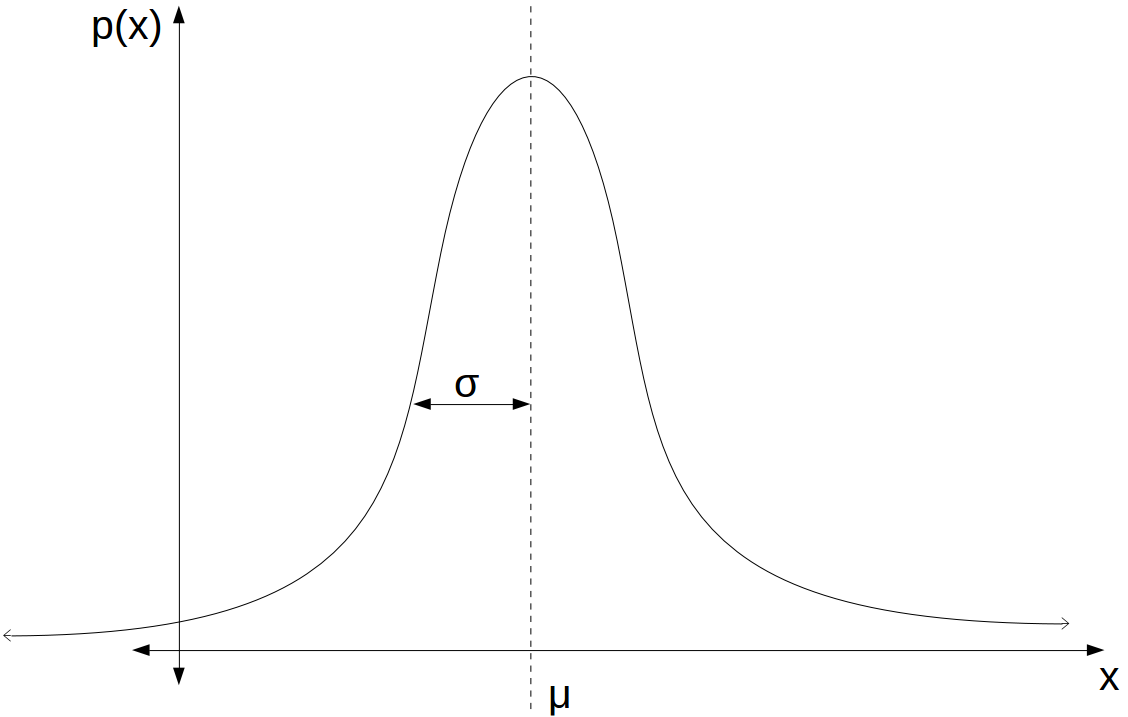
\includegraphics[width=0.7\linewidth]{Figures/univariate.png}
  \centering
  \caption{Univariate Gaussian PDF}
  \label{fig:gPDF1}
\end{figure}

\subsection{Multivariate Gaussians}
The multivariate Gaussian distribution is described by an $n$-dimensional mean vector $\bm{\mu}$ and an $n\times n$ covariance matrix $\Sigma$. The multivariate Gaussian distribution is commonly described by the following function 
\begin{equation}\label{eq:3}
p(x) = \mathcal{N}(\bm{\mu};\Sigma) = \eta\exp\left[-\frac{1}{2}(\bm{x}-\bm{\mu})^T\Sigma^{-1}(\bm{x}-\bm{\mu})\right]
\end{equation}
with normalisation coefficient
\begin{equation}\label{eq:4}
\eta = \frac{1}{(2\pi^{n/2)}|\Sigma|^{\frac{1}{2}}}
\end{equation}
$|\Sigma|$ is the the determinant of $\Sigma$
It is important that the determinant of $\Sigma$ is nonzero for the equation above to be valid. It is a requirement that $\Sigma$ is positive definite and therefore also non-singular, which guarantees a  determinant that is nonzero. In this paper we focus on positive definite covariance matrices, as it is invertible, consequentially one can use the alternative canonical or information parameterization. The canonical form is discussed in the following section.\\
The mean and covariance can sequentially be found by calculating the first and second moments of the Gaussian distribution.\\
The mean is equal to the first moment:
\begin{equation}
\bm{\mu} = \bm{E}\left[\bm{X}\right]
\end{equation}
The covariance is equal to the second moment:
\begin{equation}
\Sigma = \bm{E}[\bm{XX}]^T - \bm{E}[\bm{X}]\bm{E}[\bm{X}]^T
\end{equation}
\subsection{Error ellipse}
Multivariate Gaussian distributions can be visualized as a series of ellipsoidal contours around the mean vector $\bm{\mu}$. The contours are parallel to each other and the distance between contours suggests the steepness of the density function. The steepness of the density function is determined by the covariance matrix $\Sigma$.\\
In the following chapters it is important to show the uncertainty of PDFs, a plot of an error ellipses is an effective way to illustrate this.

\subsubsection{Eigenvalue decomposition}
The following section is based on an article from H Abdi ~\cite{abdi}.\\
In order to plot an error ellipse, the directions the covariance varies the most and the variances in those directions are needed.\\
We can use eigenvalue decomposition to factorize the covariance matrix $\Sigma$ in terms of its eigenvalues $\Lambda$ and its eigenvectors $Q$.
\begin{equation}
\Sigma = Q\Lambda Q^{-1}
\end{equation}
Each column of the eigenvector matrix $Q$ contains an eigenvector $\bm{v}$. The eigenvectors indicate the direction which the covariance varies the most. Each eigenvector has a corresponding eigenvalue $\lambda$ which specifies the variance in the direction of the eigenvector. 
\subsubsection{Plotting a 2D error ellipse}
The following section is based on a webpage from "Computer vision for dummies"~\cite{draw_ellipse}.\\
Error ellipsis are specified in terms of the confidence or probability that a random data point will fall inside the ellipse.\\To plot an error ellipse, the major - and minor axes' lengths are sequentially specified as $2\sqrt{s\lambda_1}$ and $2\sqrt{s\lambda_2}$, where $\lambda_1$ and $\lambda_2$ represent the eigenvalues of the covariance matrix ($\lambda_1 \geq \lambda_2$). For a 95\% confident ellipse $s$ is set to 5.991. If we are interested in other confidence intervals, the Chi-Sqaure distribution can be used to find an $s$ that less than or equal to a specific value which correlates with the probability of the confidence interval.\\
To obtain the orientation $\alpha$ of the error ellipse, we calculate the angle of the largest eigenvector relative to the x-axis.
\begin{equation}
\alpha = \arctan\left(\frac{\bm{v_1}(y)}{\bm{v_1}(x)}\right)
\end{equation}
In the case of an uncorrelated covariance, the eigenvalues are equal to the variances of the covariance matrix and the eigenvectors are in the same direction as the x-axis and y-axis.
\begin{figure}
  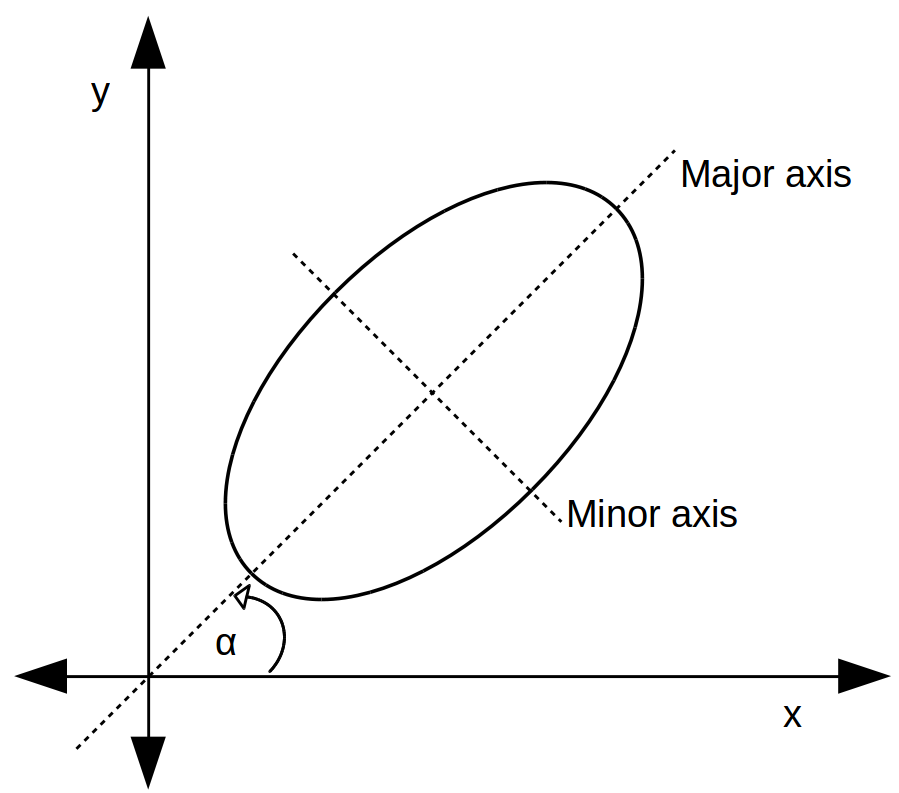
\includegraphics[width=0.6\linewidth]{Figures/e_ellipse.png}
  \centering
  \caption{Error Ellipse}
  \label{fig:e_ellipse}
\end{figure}
Figure \ref{fig:e_ellipse} shows $\alpha$ and indicates the major and minor axes of the error ellipse.

\section{Canonical form}
Linear Gaussian CPDs (conditional probability densities) are generally not Gaussians. It will be handy to find general representation that accommodates both Gaussian distributions and linear Gaussian models. The canonical or information form is a viable option. It is also much easier to perform certain operations in the canonical form. The following section is based on the work of Koller and Friedman~\cite{koller} and JC Schoeman~\citep{JC}.

\begin{equation}\label{eq:canonical}
\mathcal{C}(\bm{X}; K,\bm{h},g) = \exp\left(-\frac{1}{2}\bm{X}^TK\bm{X} + \bm{h}^T\bm{X} +g \right)
\end{equation}


It is possible to represent every Gaussian as a canonical form. Equation \ref{eq:3} can be rewritten:


\begin{multline}\label{eq:6}
\eta\exp\left[-\frac{1}{2}(\bm{x}-\bm{\mu})^T\Sigma^{-1}(\bm{x}-\bm{\mu})\right]
\\ = \exp\left(-\frac{1}{2}\bm{x}^T\Sigma^{-1}\bm{x} + \bm{\mu}^T\Sigma^{-1}\bm{x} - \frac{1}{2}\bm{\mu}^T\Sigma^{-1}\bm{\mu} + \ln{\eta}\right)
\end{multline}


$\mathcal{N}(\bm{\mu}; \Sigma) = \mathcal{C}(K,\bm{h}, g)$ by comparing \ref{eq:6} with \ref{eq:canonical}

\begin{equation}\label{eq:7}
K = \Sigma^{-1}
\end{equation}
\begin{equation}\label{eq:8}
\bm{h} = \Sigma^{-1}\bm{\mu}
\end{equation}
\begin{equation}\label{eq:9}
g = - \frac{1}{2}\bm{\mu}^T\Sigma^{-1}\bm{\mu} + \ln{\eta}
\end{equation}
$\bm{h}$ is called the potential vector and $K$ is called the information matrix.\\\\
The covariance parameters can again be recovered
\begin{equation}
\Sigma = K^{-1}
\end{equation}
\begin{equation}
\bm{\mu} = \Sigma\bm{h}
\end{equation}
The covariance form is not defined when K is not invertible, even though the distribution can still be represented in the canonical form. The canonical form is only a valid Gaussian density if and only if $K$ (information matrix) is symmetric and positive definite. The canonical form is therefore more general than the covariance form. The canonical form is very useful to present linear Gaussian CPDs. From \ref{eq:9} it can be seen that only $K$ and $\bm{h}$ are necessary to calculate $g$. Thus, $g$ can be omitted when working in the canonical form. \\


\subsection{Operations using the canonical form}
The main advantage of using the canonical form is that it is very easy to perform various operations on distributions. The variable $g$ is included in the following operations for completeness sake, but can be omitted as stated above.\\
Extending and rearranging scopes of canonical forms may be necessary before doing operations, as it is important that scopes of canonical forms are identical when doing operations.
\subsubsection{Extending the scope of a canonical form:}
If additional variables are needed, the scope of a canonical form can be extended by adding zero entries to $K$, $\bm{h}$ and $g$. 
\begin{multline}
\mathcal{C}\left(
\begin{bmatrix}
x\\
y
\end{bmatrix}:
\begin{bmatrix}
k_{xx} & k_{xy}\\
k_{yx} & k_{yy}
\end{bmatrix},
\begin{bmatrix}
h_x\\
h_y
\end{bmatrix},
\begin{bmatrix}
g_x\\
g_y
\end{bmatrix}
\right)
\\=
\mathcal{C}\left(
\begin{bmatrix}
x\\
y\\
z
\end{bmatrix}:
\begin{bmatrix}
k_{xx} & k_{xy} & 0\\
k_{yx} & k_{yy} & 0\\
0 & 0 & 0
\end{bmatrix},
\begin{bmatrix}
h_x\\
h_y\\
0
\end{bmatrix},
\begin{bmatrix}
g_x\\
g_y\\
0
\end{bmatrix}
\right)
\end{multline}
\subsubsection{Rearranging the scope of a canonical form:}
The order of the scope can be rearranged by rearranging the rows and columns of $K$  and rearranging the entries of $\bm{h}$ and $g$.
\begin{multline}
\mathcal{C}\left(
\begin{bmatrix}
x\\
y\\
z
\end{bmatrix}:
\begin{bmatrix}
k_{xx} & k_{xy} & k_{xz}\\
k_{yx} & k_{yy} & k_{yz}\\
k_{zx} & k_{zy} & k_{zz}
\end{bmatrix},
\begin{bmatrix}
h_x\\
h_y\\
h_z
\end{bmatrix},
\begin{bmatrix}
g_x\\
g_y\\
g_z
\end{bmatrix}
\right)
\\=
\mathcal{C}\left(
\begin{bmatrix}
y\\
x\\
z
\end{bmatrix}:
\begin{bmatrix}
k_{yy} & k_{yx} & k_{yz}\\
k_{xy} & k_{xx} & k_{xz}\\
k_{zy} & k_{zx} & k_{zz}
\end{bmatrix},
\begin{bmatrix}
h_y\\
h_x\\
h_z
\end{bmatrix},
\begin{bmatrix}
g_y\\
g_x\\
g_z
\end{bmatrix}
\right)
\end{multline}
\subsubsection{Multiplication of canonical forms:}
When multiplying two canonical forms, it is important that their scopes are identical. Multiplying canonical forms with the same scope is simply:
\begin{equation}\label{eq:10}
\mathcal{C}(K_1,\bm{h_1},g_1)\times\mathcal{C}(K_2,\bm{h_2},g_2) = \mathcal{C}(K_1 + K_2,\bm{h_1} + \bm{h_2},g_1 + g_2)
\end{equation}
\subsubsection{Division of canonical forms:}
Again, it important that the scopes of the distributions are identical.
\begin{equation}\label{eq:11}
\frac{\mathcal{C}(K_1,\bm{h_1},g_1)}{\mathcal{C}(K_2,\bm{h_2},g_2)} = \mathcal{C}(K_1 - K_2,\bm{h_1} - \bm{h_2},g_1 - g_2)
\end{equation}
\subsubsection{Marginalization of a canonical form:}
A marginal distribution can be found by integrating over a subset of variables. For example the marginal distribution over $\bm{X}$ can be found by integrating over $\bm{Y}$.\\
Let $\mathcal{C}(\bm{X},\bm{Y};K,\bm{h},g)$ be a canonical form with subsets $\bm{X}$ and $\bm{Y}$ where
\begin{equation}
K = 
\begin{bmatrix}
K_{\bm{XX}} & K_{\bm{XY}}\\
K_{\bm{XY}} & K_{\bm{YY}}
\end{bmatrix}
 ; h = 
\begin{pmatrix}
h_{\bm{X}} \\
h_{\bm{Y}}
\end{pmatrix}
\end{equation}
To obtain the marginal distribution over $\bm{X}$, we have to find the integral over $\bm{Y}$. Therefore
\begin{equation}
\int\mathcal{C}(\bm{X},\bm{Y};K,\bm{h},g)d\bm{Y} = \mathcal{C}(\bm{X};K',\bm{h}',g')
\end{equation}
 where
\begin{equation}
K' = K_{\bm{XX}} - K_{\bm{XY}}K_{\bm{XY}}^{-1}K_{\bm{YX}}
\end{equation}
\begin{equation}
h' = \bm{h}_{\bm{X}} - K_{\bm{XX}}K_{\bm{YY}}^{-1}\bm{h}_{\bm{Y}}
\end{equation}
\begin{equation}
g' = g - \frac{1}{2}\left(\ln|2\pi K_{\bm{YY}}^{-1}|+ \bm{h_Y}^T K_{\bm{YY}}^{-1}\bm{h_Y}\right)
\end{equation}
It is important to that $K_{\bm{YY}}$ is positive-definite for the result to be finite.
\subsubsection{Reduction with evidence:}
Let $\mathcal{C}(\bm{X},\bm{Y};K,\bm{h},g)$ be a canonical form with subsets $\bm{X}$ and $\bm{Y}$. If subset $\bm{Y}$ is known $(\bm{Y} =  \bm{y})$, then the canonical form can be reduced to $\mathcal{C}(\bm{X}; K',\bm{h}',g')$, where
\begin{equation}
K' = K_{\bm{XX}}
\end{equation}
\begin{equation}
h' = \bm{h}_{\bm{X}} - K_{\bm{XY}}\bm{y}
\end{equation}
\begin{equation}
g' = g + \bm{h}_{\bm{Y}}^T\bm{y} - \frac{1}{2}\bm{y}^TK_{\bm{YY}}\bm{y}
\end{equation}
\subsection{Using the canonical form the present conditional distributions (linear transformations)}
The following section is based on a skripsie from JC Schoeman~\cite{JC} and notes from Dr CE van Daalen. One of the advantages of the canonical form is that it is possible to present conditional probability distributions (CPDs). \\
If a CPD such as $p(\bm{y}|\bm{x})$ can be described as a linear transform:
\begin{equation}
\bm{y} = F\bm{x} + \bm{g} + \bm{n}
\end{equation}
where
\begin{equation}
n = \mathcal{N}(\bm{0}, \Sigma_n)
\end{equation}
\begin{equation}
\label{eq:30}
\begin{split}
p(\bm{y}|\bm{x}) & = \mathcal{N}(F\bm{x} + \bm{g}, \Sigma) \\
& = \eta\exp\left[-\frac{1}{2}(\bm{y} - (F\bm{x} + \bm{g}))^T\Sigma^{-1}(\bm{y}-(F\bm{x} + \bm{g}))\right]
\end{split}
\end{equation}
Rewriting
\begin{equation}
\begin{split}
\bm{y} - (F\bm{x} + \bm{g}) & =
\begin{bmatrix}
I&-F&-I
\end{bmatrix}
\begin{bmatrix}
\bm{y}\\
\bm{x}\\
\bm{g}
\end{bmatrix}\\
& =
\begin{bmatrix}
I\\-F^T\\-I
\end{bmatrix}^T
\begin{bmatrix}
\bm{y}\\
\bm{x}\\
\bm{g}
\end{bmatrix}\\
\end{split}
\end{equation}
Equation \ref{eq:30} becomes
\begin{equation}
\label{eq:32}
\begin{split}
p(\bm{y}|\bm{x}) = \eta\exp\left[-\frac{1}{2}
\begin{bmatrix}
\bm{y}\\
\bm{x}\\
\bm{g}
\end{bmatrix}^T
\begin{bmatrix}
I\\-F^T\\-I
\end{bmatrix}
\Sigma^{-1}
\begin{bmatrix}
I\\-F^T\\-I
\end{bmatrix}^T
\begin{bmatrix}
\bm{y}\\
\bm{x}\\
\bm{g}
\end{bmatrix}
\right]
\end{split}
\end{equation}
Defining a combined random vector
\begin{equation}
\bm{w} = 
\begin{bmatrix}
\bm{y}\\
\bm{x}\\
\bm{g}

\end{bmatrix}
\end{equation}
and information matrix
\begin{equation}
K' =
\begin{bmatrix}
I\\-F^T\\-I
\end{bmatrix}
\Sigma^{-1}
\begin{bmatrix}
I\\-F^T\\-I
\end{bmatrix}^T
\end{equation}
Equation \ref{eq:32} can be rewritten
\begin{equation}
\label{eq:35}
\begin{split}
p(\bm{y}|\bm{x}) = \eta\exp\left[-\frac{1}{2}
\bm{w}^T
K'
\bm{w}
\right]
\end{split}
\end{equation}
This closely relates with the canonical form in equation \ref{eq:canonical}
\begin{equation}
\begin{split}
p(y|x) & = \mathcal{C}(\bm{w}: K', \bm{0})\\
& =\mathcal{C}\left(
\begin{bmatrix}
\bm{y} \\
\bm{x} \\
\bm{g}
\end{bmatrix};
\begin{bmatrix}
I\\
-F^T\\
-I
\end{bmatrix}
\Sigma_n^{-1}
\begin{bmatrix}
I & -F & -I
\end{bmatrix}, \bm{0}, -
\right)\\
& =\mathcal{C}\left(
\begin{bmatrix}
\bm{y} \\
\bm{x} \\
\end{bmatrix};
\begin{bmatrix}
I\\
-F^T
\end{bmatrix}
\Sigma_n^{-1}
\begin{bmatrix}
I & -F
\end{bmatrix},
\begin{bmatrix}
I\\
-F^T
\end{bmatrix}
\Sigma_n^{-1}\bm{g}, -
\right)\\
& =\mathcal{C}\left(
\begin{bmatrix}
\bm{y} \\
\bm{x} \\
\end{bmatrix};
\begin{bmatrix}
\Sigma_n^{-1}  &  -\Sigma_n^{-1}F\\
-F^T\Sigma_n^{-1} & F^T\Sigma_n^{-1}F
\end{bmatrix}
, 
\begin{bmatrix}
-\Sigma_n^{-1}\bm{g}\\
-F^T\Sigma_n^{-1}\bm{g}
\end{bmatrix},
-
\right)
\end{split}
\end{equation}
\chapter{Localisation using Kalman Filters}
\section{Kalman Filter}
\section{Motion models}
\section{Measurement models}
\section{Extended Kalman Filter}
\section{Unscented Kalman Filter}
\chapter{Probabilistic Graphical Models}
This chapter gives a brief introduction to Probabilistic Graphical Models (PGMs). PGMs are a very vast field which is beyond the scope of this document, therefore only the theory relevant to this paper will be covered. This chapter is based on the work of Koller and Friedman~\cite{koller}, Barber~\cite{barber} and Schoeman~\citep{JC}.
\section{Overview}
Reasoning about systems with uncertainty can become very complex and sometimes seems to be completely unmanageable. The PGM is a graphical technique which allows to construct probabilistic systems in a logical and compact manner which makes problems tractable. PGMs are thus used to describe the relationship between RVs and allows to reason about them. (note the action of querying a system is called inference) These relationships are usually in the form of conditional probability densities (CPDs). It is a very popular technique, as it is intuitive, transparent and easy to manipulate. PGMs have limitations such as image recognition, where neural networks thrive.\\
PGMs can be divided in to two categories. The first is Markov networks, which uses directed graphs. The second is Bayesian networks, which uses undirected graphs. Markov networks are used for non-causal systems and Bayesian networks are used for causal systems. In most cases the localisation problem is causal, thus Bayesian networks are used in this paper and the focus is on directed graphs.\\
Continuous RVs are used to describe PGMs in this paper, as it is applicable for localisation. PGMs have countless applications from making medical diagnosis to localising robots.
\section{Basic concepts of graphical models}
A graph consists of nodes and edges. Edges are the link between nodes and can be undirected or directed. If all edges are undirected then the graph is classified as undirected. If all edges are directed, then the graph is classified as directed. If there is an edge in the direction from A to B, as in Figure \ref{fig:comGraphs} (b), then A is a parent of B and B is a child of A.
\begin{figure}[h!]
  \centering
  \begin{subfigure}[b]{0.3\linewidth}
    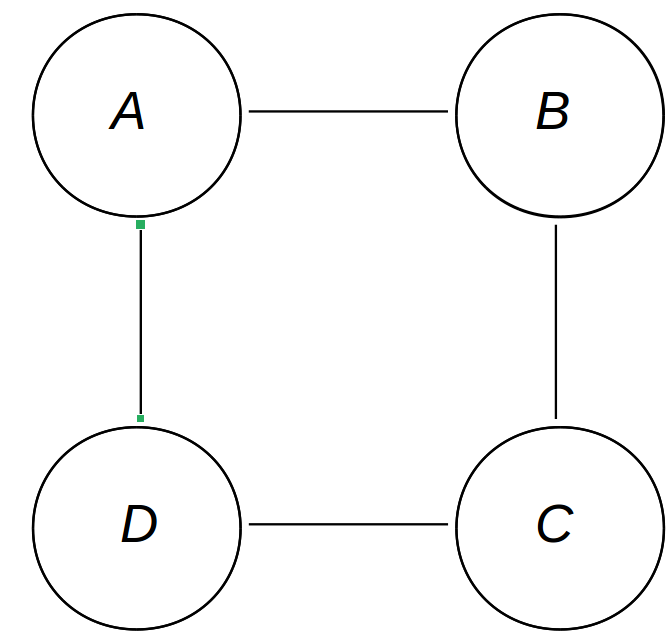
\includegraphics[width=\linewidth]{Figures/undirected_graph.png}
    \caption{Undirected graph}
  \end{subfigure}
  \begin{subfigure}[b]{0.3\linewidth}
    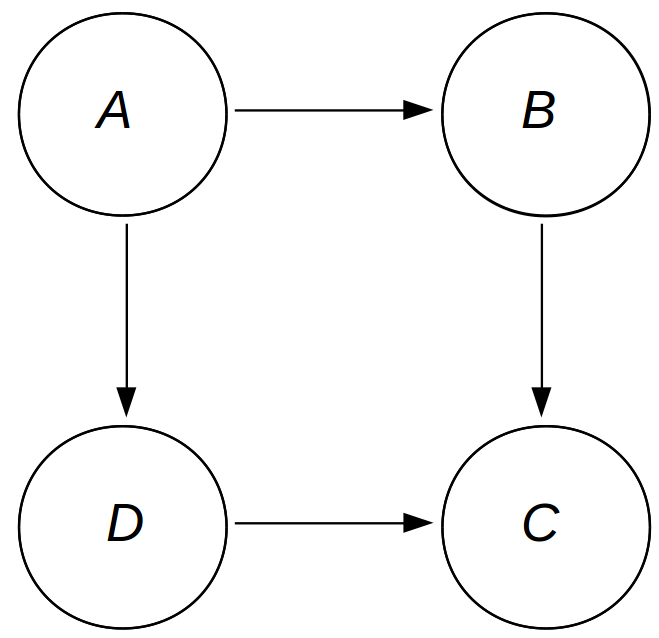
\includegraphics[width=\linewidth]{Figures/directed_graph.png}
    \caption{Directed graph}
  \end{subfigure}
  \caption{}
  \label{fig:comGraphs}
\end{figure}
\section{Bayesian PGMs}
\begin{figure}[H]
  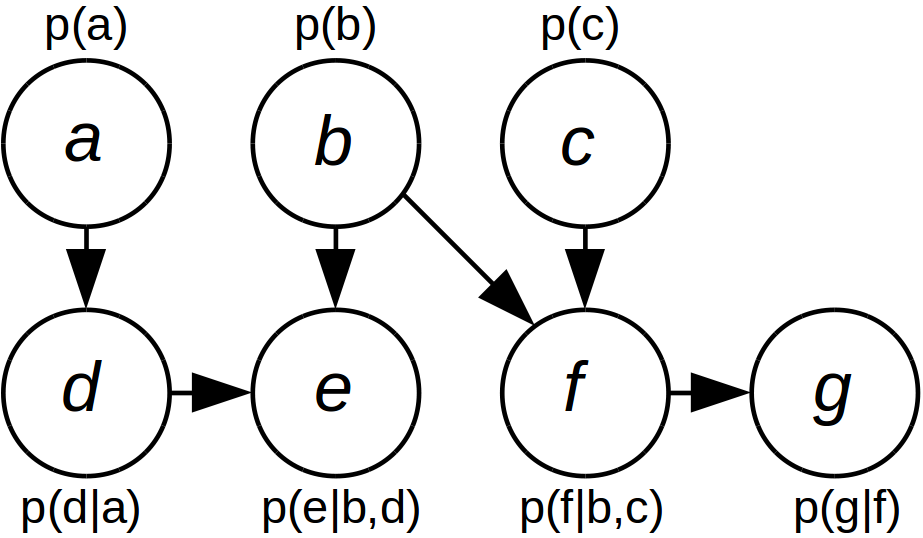
\includegraphics[width=0.6\linewidth]{Figures/bayesian_pgm.png}
  \centering
  \caption{Bayesian PGM}
  \label{fig:bays_pgm}
\end{figure}
\begin{equation}
p(a,b,c,d,e,f,g) = p(a)p(b)p(c)p(d|a)p(e|b,d)p(f|b,c)p(g|f)
\end{equation}
\section{Inference with cluster graphs}
\begin{figure}[H]
  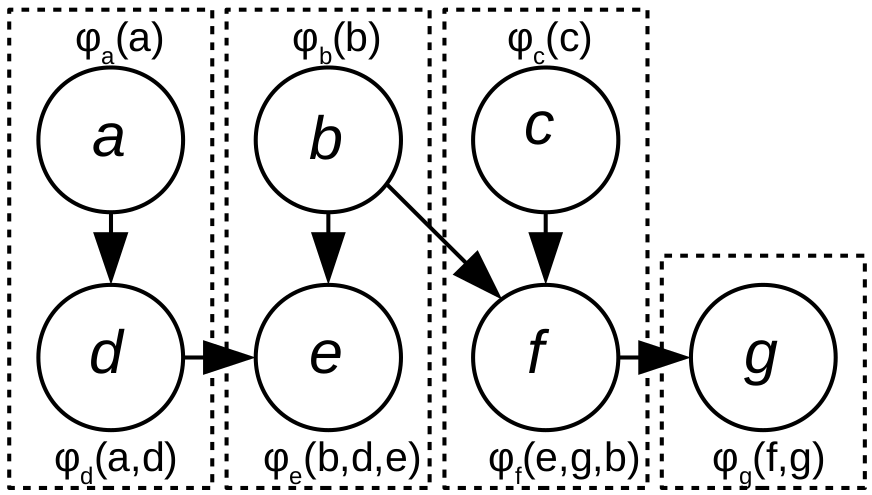
\includegraphics[width=0.6\linewidth]{Figures/cluster_divisions.png}
  \centering
  \caption{Bayesian PGM with cluster boundaries}
  \label{fig:e_ellipse}
\end{figure}
\begin{figure}[H]
  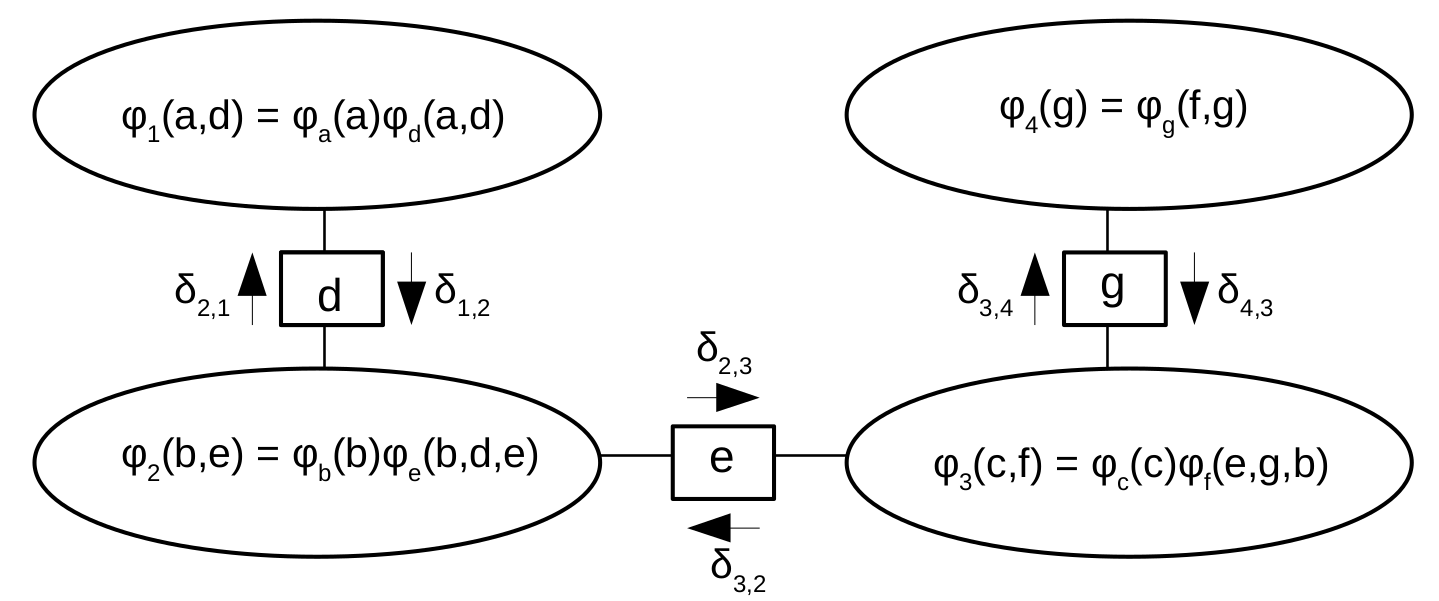
\includegraphics[width=\linewidth]{Figures/clustergraph.png}
  \centering
  \caption{Cluster graph}
  \label{fig:e_ellipse}
\end{figure}
\section{Message passing}
\chapter{Localisation using Probabilistic Graphical Models}
\section{Linear localisation}
\section{Non-linear localisation}
\subsection{Taylor series expansion}
\subsection{Unscented transform}
\subsection{Monte Carlo integration}

\backmatter
\bibliography{mybib}{}

\end{document}\grid
